%%%%%%%%%%%%%%%%%%%%%%%%%%%%%%%%%%%%%%%%%%%%%%%%%%%%%%%%%%%%%%%%%%%%%%%%%%%%%%%%%%%%%%%%%%%%%%%%
%
% CSCI 1430 Written Question Template
%
% This is a LaTeX document. LaTeX is a markup language for producing documents.
% Your task is to answer the questions by filling out this document, then to
% compile this into a PDF document.
%
% TO COMPILE:
% > pdflatex thisfile.tex

% If you do not have LaTeX, your options are:
% - VSCode extension: https://marketplace.visualstudio.com/items?itemName=James-Yu.latex-workshop
% - Online Tool: https://www.overleaf.com/ - most LaTeX packages are pre-installed here (e.g., \usepackage{}).
% - Personal laptops (all common OS): http://www.latex-project.org/get/ 
%
% If you need help with LaTeX, please come to office hours.
% Or, there is plenty of help online:
% https://en.wikibooks.org/wiki/LaTeX
%
% Good luck!
% The CSCI 1430 staff
%
%%%%%%%%%%%%%%%%%%%%%%%%%%%%%%%%%%%%%%%%%%%%%%%%%%%%%%%%%%%%%%%%%%%%%%%%%%%%%%%%%%%%%%%%%%%%%%%%
%
% How to include two graphics on the same line:
% 
% \includegraphics[width=0.49\linewidth]{yourgraphic1.png}
% \includegraphics[width=0.49\linewidth]{yourgraphic2.png}
%
% How to include equations:
%
% \begin{equation}
% y = mx+c
% \end{equation}
% 
%%%%%%%%%%%%%%%%%%%%%%%%%%%%%%%%%%%%%%%%%%%%%%%%%%%%%%%%%%%%%%%%%%%%%%%%%%%%%%%%%%%%%%%%%%%%%%%%

\documentclass[10pt,twocolumn,letterpaper]{article}
 
\usepackage{cvpr}
\usepackage{times}
\usepackage{epsfig}
\usepackage{graphicx}
\usepackage{amsmath}
\usepackage{amssymb}
\usepackage{booktabs}
\usepackage{microtype}
% From https://ctan.org/pkg/matlab-prettifier
\usepackage[numbered,framed]{matlab-prettifier}

\frenchspacing

% Include other packages here, before hyperref.

% If you comment hyperref and then uncomment it, you should delete
% egpaper.aux before re-running latex.  (Or just hit 'q' on the first latex
% run, let it finish, and you should be clear).
\usepackage[pagebackref=true,breaklinks=true,letterpaper=true,colorlinks,bookmarks=false]{hyperref}

\cvprfinalcopy
\def\cvprPaperID{****}
\def\httilde{\mbox{\tt\raisebox{-.5ex}{\symbol{126}}}}
\ifcvprfinal\pagestyle{empty}\fi

\begin{document}

%%%%%%%%% TITLE
\title{CSCI 1430 Final Project Report:\\NFL Position Classification Through YOLO}

% Make this document not anonymous
\author{
    \emph{The Playmakers}: John Michael Slezak, Atif Khan, Chenhao Lu, Ruida Zeng.\\
    \emph{TA name:} Joel Manasseh.
    Brown University\\
}

\maketitle
%\thispagestyle{empty}

%%%%%%%%% ABSTRACT
\begin{abstract}
Object classification is a pivotal development in computer vision with applications in medicine, autonomous vehicles, and many more. The purpose of this study is to investigate how context and place within an image can affect a models ability to classify an object. This problem is studied through an analysis of position labeling on a football field where the players have no distinguishing characteristics between them. Thus, the model has to learn from the context and location of the features versus the features themselves to classify them. For these purposes, a custom dataset of NFL formations were gathered and labeled. Then the object detection algorithm YOLO(You Only Look Once) was implemented for training the model. The results varied as the model did a reasonable job classifying wide receivers and cornerbacks. However, it struggled with identifying safetys and the fact that referees were not players. In summary, this model did a reasonable job, but could have been helped by access to more data. 
\end{abstract}


%%%%%%%%% BODY TEXT
\section{Introduction}


In this project, we are trying to build an algorithm that can identify the positions of players on an NFL field before the play begins. This problem is difficult because of the similarities between the players when compared with other object classification implementations. All of the players are humans in NFL equipment. Thus, when compared to classifying objects like apples and oranges, context must be taken into account much more than just the features of the object itself. Also, players line up as different positions depending on the play itself. For this project, we classified players based on how they lined up, not their preset position on a depth chart. 
We will implement YOLO, You Only Look Once, for object identification on a custom dataset created by us using Roboflow labeling software. This type of algorithm would be very helpful for sports analytics, especially, with tracking software once it is started so as to tracks plays and players in real time. More analysis could be done on said plays to both improve the sport and gameplay. In addition to its application to sports, this progress in moving from feature identification to context and location within an image could help future obect detection algorithms in various fields.

\section{Related Work}

When first researching which computer vision model to train, we came across various options. However, YOLO turned out to be the best option after reading many research papers on it.
One of the main strengths of YOLO is that it is extremely fast and makes fewer background errors than traditional R-CNN approaches.~\cite{Alpher05} Prava et al. Furthermore, 
the specific version of YOLO we used was YOLOv8. The reason we used this version of YOLO, other than it being a massive improvement from previous versions, is that YOLOv8 was used for UAV aerial photography scenarios which is a similar scenario to NFL plays due to the top-down
view of the field.~\cite{Alpher02} Jiang et al. Lastly, although we needed a fast model that didn't require a lot of time and resources to train, we also didn't want to sacrifice accuracy. Faster R-CNN achieves, one of the most accurate object detection models, achieved a mean accuracy precision score of 76.8 with a Frame Per Second score of 5 to 18.~\cite{Du_2018} Juan Du. Although
it is extremely accurate, it is very slow. Comparatively, YOLO achieved a mean accuracy precision score of 78.6 and a blazing fast Frame Per Second score of 155.~\cite{Du_2018} Juan Du. And so, with all of this research in mind, we decided to choose YOLOv8 for our model.

\section{Method}

Before an NFL play begins, all of the players line up in formation on both the offensive and defensive side of the ball. We wanted to find out if we could train a model to be able to recognize what position each player was lined up as. Our approach was to build a custom dataset and train a model on it. We first went through the 2024 Super Bowl, and the AFC and NFC championship for that year documenting every presnap formation. After that we used Roboflow software to label the positions for all 503 images, excluding the offensive and defensive lines. Below is an example after labeling.~\cite{Roboflow}
\begin{figure}[t]
    \centering
    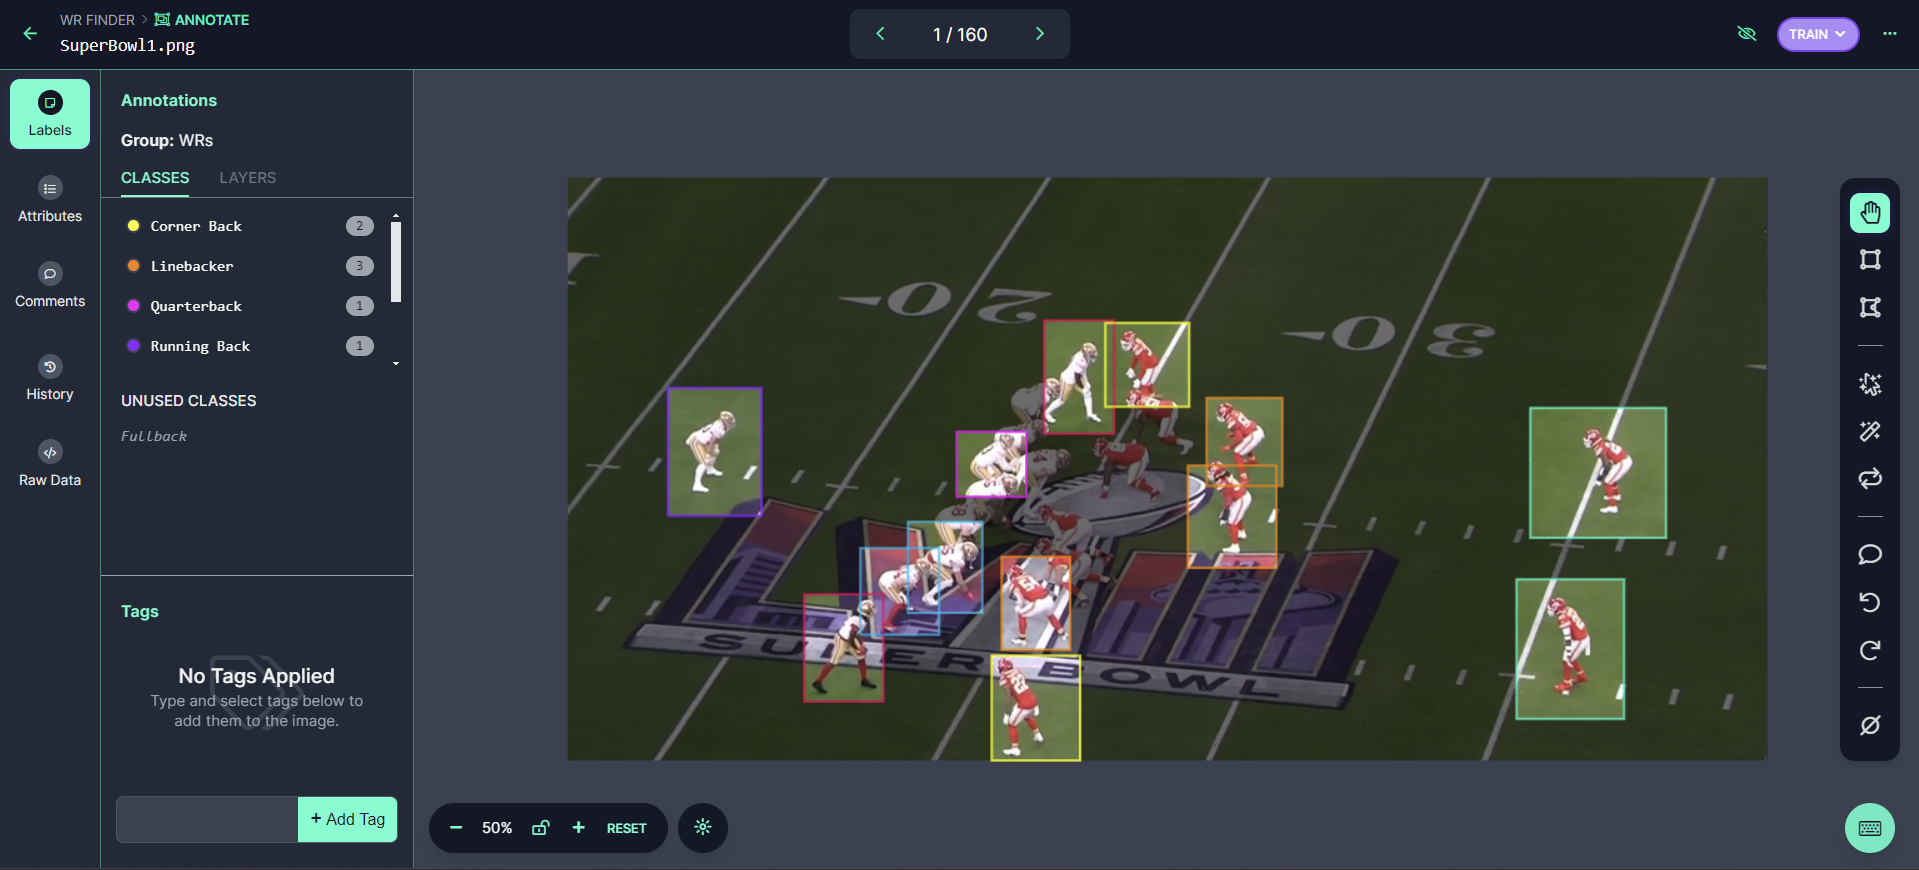
\includegraphics[width=\linewidth]{LabelingExample.png}
    \caption{Labeling Example}
    \label{fig:result1}
\end{figure}

\subsection{Color Matching}
The first detection method we tried was direct color matching, and the idea was to use uniquely identifiable colors of each team to detect players (e.g. gold for SF, red for KC), and identify the wide receivers based on the position of the bounding boxes. We first converted the image from RGB to LAB to take into account the luminance factor, and computed the distance between each pixel and the LAB values of gold and red. We then applied thresholding to keep only pixels within an arbitrary distance and converted the image to binary. With OpenCV's blob detection methods, we were able to detect potential player regions and keep the ones larger than an arbitrary size.

In order to know what color to match, we need to know which side is the offensive side. To do that, we utilized the assumption that an offensive formation is usually narrower horizontally than a defensive formation, i.e. players are closer together. For each team, we computed the distance between the x coordinates of the leftmost and rightmost bounding boxes, and the team with a smaller distance will be the offensive team.

To identify wide receivers, we then simply looked for the bounding boxes with the largest and smallest y coordinates, i.e. closer to the horizontal image edges. 

\subsection{Detection Using YOLO}
After accomplishing this on the 503 images from the three games, we exported them in the YOLOv8 format, so as to use that algorithm to do the object detection.
The model that we used is called YOLOv8 (You Only Look Once). The way that YOLO works is that it processes an entire image in one go, unlike other systems that analyze parts of the image sequentially. This whole image processing allows YOLO to quickly detect objects.
To localize objects precisely, the image is divided into a grid. Each grid section predicts the presence, shape, and size of objects within it. For each detected object, YOLO assigns a confidence score that indicates the certainty of the object’s presence and the accuracy of the bounding box that outlines it. To ensure the most accurate results, YOLO employs a technique known as non-max suppression, which refines these bounding boxes by keeping only the most precise predictions and eliminating any overlaps or redundancies. The final output is an image annotated with boxes and labels around each detected object, clearly identifying and locating them within the scene. Figure \ref{fig:architecture} below shows the architecture of YOLOv8.

In the context of labeling NFL players on the field, as the image of the football field is processed in a single glance, it's divided into a grid, where each section of the grid is tasked with identifying and labeling the players within its bounds. YOLO predicts the presence and exact location of each player, assigning labels such as quarterback, receiver, or lineman based on their positions relative to others and the game's context. Each prediction includes a bounding box around the player with a confidence score that indicates the accuracy of both the player's identification and position. Moreover, using techniques like non-max suppression, YOLO ensures that each player is uniquely identified and labeled only once, even in crowded scenes, resulting in a clear and accurate depiction of all player positions on the field. 
\begin{figure*}[t]
    \centering
    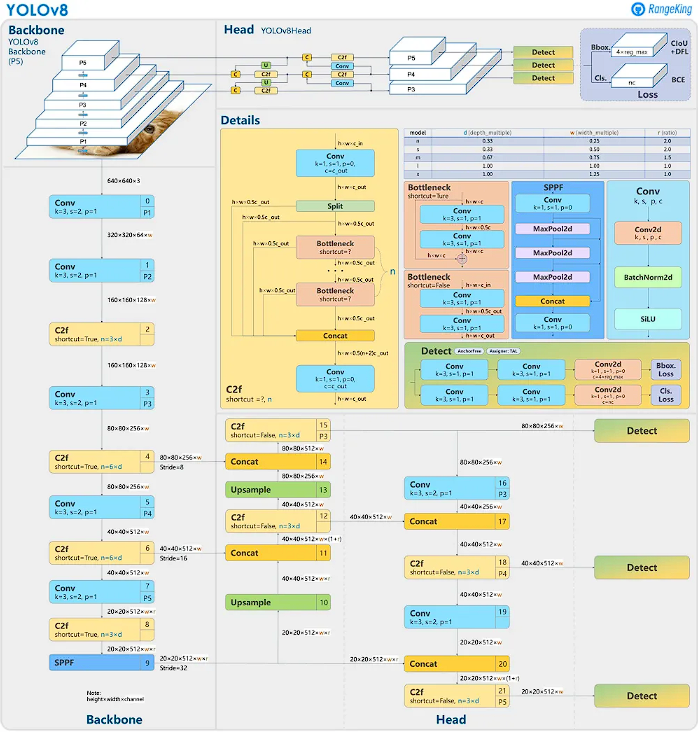
\includegraphics[width=0.8\linewidth]{architecture.png}
    \caption{YOLOv8's architecture. \href{https://blog.roboflow.com/whats-new-in-yolov8/}{source}}
    \label{fig:architecture}
\end{figure*}

\section{Results}

Figure \ref{fig:result2} below shows the results of the color matching algorithm applied on two images from the SF vs. KC super bowl game. The right image is a correct identification of the wide receivers. In the left image, the algorithm failed to identify the offensive team.

\begin{figure*}[t]
    \centering
    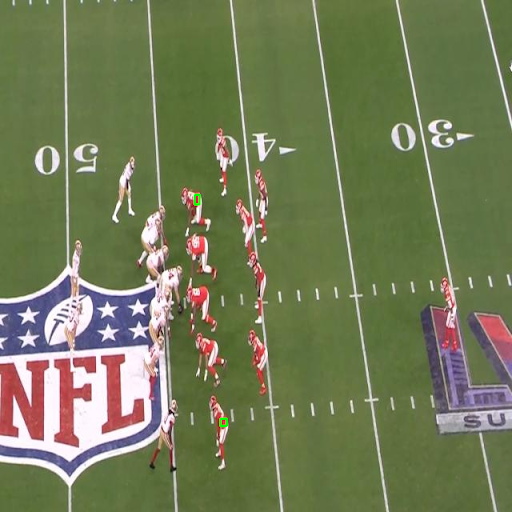
\includegraphics[width=0.4\linewidth]{color_matching_1.png}
    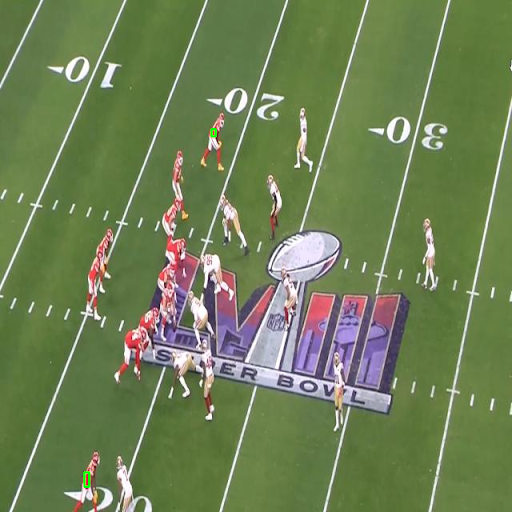
\includegraphics[width=0.4\linewidth]{color_matching_2.png}
    \caption{Examples of the wide receivers detected using color matching.}
    \label{fig:result2}
\end{figure*}

%-------------------------------------------------------------------------
\subsection{Technical Discussion}

Despite successfully identifying the wide receivers, the color matching algorithm has clear limitations that made it impractical to be used. The algorithm is very sensitive to any kinds of background noises, e.g. the NFL logo, end zones, yard numbers, etc. It's also not very generalizable because we need to know exactly what color to use to identify each team. Finally, the algorithm only matches specific parts of the players, instead of the entire player. Depending on the angle and body position of the players, some color features will not be detectable. For example, if the player’s jersey is blocked by his arm or another players, the color matching algorithm will no longer be able to detect the jersey. These limitations are the reasons why we switched to a model-based YOLO detection pipeline.

We chose YOLO for identifying positions of NFL players on the field because it has a blend of efficiency, accuracy, and practical applicability which made it suitable for this specific task. YOLO is renowned for its speed, which allows real-time processing and is a significant advantage when working with limited CPU/GPU resources to train a model.
 Also, YOLO's architecture is designed to look at the entire image during detection, which helps it capture contextual information that is crucial for accurately identifying player positions in the dynamic environments of NFL games.
 However, there are trade-offs to consider. YOLO generally prioritizes speed over precision compared to Transformers-Based Models such as DETR and Swin Transformer, which might result in a slightly lower accuracy, particularly in densely packed scenes typical of sports events where players cluster together. This trade-off means that while YOLO can quickly process images and provide a fast response, it might require fine-tuning and possibly more training data to match the precision offered by other slower but more meticulous models.
 If we had more time and resources, ideally we would experiment with vaarious other models to see which one gives the best results.


%------------------------------------------------------------------------
\section{Conclusion}

In the end, we used the YOLO model on a custom dataset to create a model that would identify the positions of players on an NFL field. The ability to perform this analysis in real-time has many applications for the sports world and beyond. For example, being able to identify players positions and then potentially tracking their movements could help with performance analytics for both the player and the plays themselves. In addition, access to more data in sports over the years, has helped develop new techniques and outlaw plays that were particularly harmful to players safety. The ability to track how formations affect injury risk could open up another pathway to help players remain healthy. Lastly, we found that how YOLO worked helped it analyze the full context of the image allowing for it to better identify the players. Designing and building models that take into account context will help with many future object classification algorithms regardless of the use case. The entire sports and media industry is a massive component of the world economy. Imporoving the games and keeping athletes healthy while they play and after they retire is a huge endeavor that needs every tool at its disposal. This position classification model will help to achieve that goal.
{\small
\bibliographystyle{plain}
\bibliography{ProjectFinal_ProjectReportTemplate}
}

\section*{Appendix}

\subsection*{Team contributions}

Please describe in one paragraph per team member what each of you contributed to the project.
\begin{description}
\item[John Michael Slezak] Created the dataset and labeled all of the images that the YOLO model was eventually trained on. Helped to write the code to train the YOLO model. Contributed to the results and methods section of the poster and the mehtods, introduction, and conclusion section of the report. 
\item[Atif Khan] Worked on writing the code and training the model for the player detection algorithm as well as researching the YOLO model. Contributed to the methods, technical discussion, and related works section of the report as well as the beginning sections of the poster.
\item [Chenhao Lu] Researched methods for object detection, wrote and tested the code for applying the pre-trained YOLO model without fine-tuning, wrote and tested the code for the color matching algorithm.
\item [Ruida Zeng] Lorem ipsum dolor sit amet, consectetur adipiscing elit, sed do eiusmod tempor incididunt ut labore et dolore magna aliqua. Ut enim ad minim veniam, quis nostrud exercitation ullamco laboris nisi ut aliquip ex ea commodo consequat. Duis aute irure dolor in reprehenderit in voluptate velit esse cillum dolore eu fugiat nulla pariatur.
\end{description}

\end{document}
